\documentclass[11pt]{article}

\newcommand{\pset}{
    3
}
\newcommand{\subtitle}{
    The Algebra of Regular Expressions;
    Kleene's Theorem;
    Silent Transitions
}
\newcommand{\duedate}{
    Friday, September 26
}

% Page Setup
\usepackage{geometry}
\geometry{
    a4paper,
    margin={2.5cm}
}

% Basic Packages
\usepackage{amssymb}
\usepackage{stmaryrd}
\usepackage{amsmath}
\usepackage{amsthm}
\usepackage{mathtools}
\usepackage{mathpartir}
\usepackage{enumitem}
\usepackage{mathabx}

% Font
\usepackage{charter}

% Bibliography and index
\usepackage[backend=biber, style=numeric]{biblatex}
\addbibresource{refs.bib}
\usepackage{makeidx}
\makeindex

% Colors and Graphics
\usepackage[dvipsnames, x11names]{xcolor}
\usepackage{tikz}
\usetikzlibrary{
    cd,
    fit,
    calc,
    positioning,
    arrows,
    automata,
    shapes
}
\tikzset{
    baseline = (current bounding box.center),
    every state/.append style = {
        rectangle,
        rounded corners=5pt,
		inner sep = 3pt,
		minimum size = 18pt,
		initial text = {},
        fill=Azure1
	},
	every edge/.append style = {
		->,
		>=stealth,
		bend angle=10,
		thick
	}
}
\usepackage{musicography}
\usepackage{graphicx}
\usepackage{svg}
\graphicspath{../imgs/}

% Hyperlinks
\usepackage{hyperref}
\hypersetup{
    colorlinks,
    linkcolor   = black,
    filecolor   = RubineRed,
    urlcolor    = RubineRed,
    citecolor   = RubineRed,
    pdftitle    = {CSCI 341 Course Materials}
}
\usepackage[capitalize]{cleveref}

% Environments
\theoremstyle{theorem} % In Italics
\newtheorem{theorem}                    {{\color{Purple}Theorem}}[section]
\newtheorem{lemma}          [theorem]   {{\color{Magenta}Lemma}}
\newtheorem{proposition}    [theorem]   {Proposition}
\newtheorem{corollary}      [theorem]   {Corollary}
\newtheorem{question}                   {{\color{red}Question}}

\theoremstyle{definition} % Not in italics
\newtheorem{definition}     [theorem]   {{\color{NavyBlue}Definition}}
\newtheorem{example}        [theorem]   {{\color{ForestGreen}Example}}
\newtheorem{problem}                    {{\color{BurntOrange}Problem}}

\theoremstyle{remark} % Subdued label
\newtheorem{remark}[theorem]        {{\color{Gray}Remark}}

% (1), (2), ...
\renewcommand\labelenumi{(\theenumi)}

% Go nuts with line breaks 
\allowdisplaybreaks

%%%%%%%%%%
% MACROS %
%%%%%%%%%%

\newcommand{\op}{\mathrm{op}}               % Opposite
\newcommand{\inv}{{-1}}                     % Inverse
\newcommand{\id}{\mathsf{id}}               % Identity f(x) = x
\newcommand{\Det}{\mathrm{Det}}             % determinize
\newcommand{\Lang}{\mathcal{L}}             % Language

\newcommand{\incl}{\mathsf{incl}}           % Inclusion
\newcommand{\proj}{\mathsf{proj}}           % Projection

% Numbers and Standard notation
\newcommand{\NN}{\mathbb{N}}                % 0, 1, 2, 3, 4, ...
\newcommand{\ZZ}{\mathbb{Z}}                % ..., -2, -1, 0, 1, 2, ...
\newcommand{\QQ}{\mathbb{Q}}                % n/m for n and m in \NN and m > 0
\newcommand{\RR}{\mathbb{R}}                % real numbers
\newcommand{\pRR}{\mathbb{R}_{+}}           % positive real numbers

\newcommand{\dom}{\mathrm{dom}}             % Domain
\newcommand{\cod}{\mathrm{cod}}             % Codomain

\newcommand{\Grph}{\operatorname{Grph}}     % Graph of a function

% Transitions
\newcommand{\tr}[1]{
    \mathrel{
        \raisebox{-1pt}{
            \(\xrightarrow{#1}\)
        }
    }
}
\newcommand{\bisim}{\mathrel{\raisebox{1pt}{\(\underline{\leftrightarrow}\)}}}

% Text
\newcommand{\code}[1]{\texttt{#1}}
\newcommand{\codeblock}[1]{
    \begin{center}
        \parbox{0.8\textwidth}{
            \ttfamily
            #1
        }
    \end{center}
}

% Boolean statements
\newcommand{\OR}{~\mathrm{or}~}
\newcommand{\AND}{~\mathrm{and}~}
\newcommand{\NOT}{\mathrm{not}~}
\newcommand{\IMPLIES}{~\mathrm{implies}~}
\newcommand{\FORALL}{\mathrm{for\ all}~}
\newcommand{\EXISTS}{\mathrm{there\ exists}~}
\newcommand{\SUCHTHAT}{~\mathrm{such\ that}~}



% Title
\title{CSCI 341 Problem Set \pset}
\author{\subtitle}
\date{Due
    \duedate
}

\begin{document}

\maketitle

Don't forget to check the webspace for hints and additional context for each problem!

\subsection*{Algebra of Regular Expressions}

\begin{problem}
    [Distributing on the Left]
    Let \(r_1,r_2,r_3 \in \mathit{RExp}\).
    Prove the equation 
    \[r_1 \cdot (r_2 + r_3) =_{\mathcal L} (r_1 \cdot r_2) + (r_1 \cdot r_3)\]
    by calculating the language on either side of the equation and arguing that these two languages are equal.   
\end{problem}

\begin{proof}[Solution.]
    
\end{proof}

\begin{problem}
    [Air Flare]
    Let \(a,b \in A\).
    Use the equations in the Lemmas above to prove the following equations:
    \begin{enumerate}
        \item \(a^*a^* =_{\mathcal L} a^*\)
        \item \((a + b)^* =_{\mathcal L} b^*(ab^*)^*\)
    \end{enumerate}
    Label each equation you use in your proof to indicate which lemma was used where.  
\end{problem}

\begin{proof}[Solution.]
    
\end{proof}

\subsection*{Kleene's Theorem}

\begin{problem}
    [Some String Matching]
    Let \(A = \{0,1\}\).
    In the following automaton, the state \(x_0\) represents a program that checks that in a given input string, every instance of \(01\) is eventually followed by a \(0\).

    \begin{figure}[h]
        \centering
        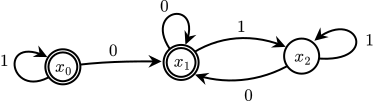
\includegraphics{01then0.pdf}
        \caption{An automaton \(\mathcal A\) with a state \(x_0\) that accepts a string of \(0\)s and \(1\)s if and only if every instance of \(01\) is eventually followed by \(0\).}
    \end{figure}

    \begin{enumerate}
        \item Use Kleene's algorithm to derive a regular expression \(s_0 \in \mathit{RExp}\) such that \(\mathcal L(\mathcal A, x_0) = \mathcal L(s_0)\).
        
        \item 
            Draw the portion of the Antimirov automaton generated by \(s_0\), \(\mathcal A' = \langle s_0\rangle_{\mathcal A_{Ant}}\). 
            There is a state \(y_0\) is the Antimirov automaton such that \(\mathcal A = \langle y_0\rangle_{\mathcal A'}\).
            Find \(y_0\).
    \end{enumerate}
\end{problem}

\begin{proof}[Solution.]
    
\end{proof}


\subsection*{Silent Transitions}

\begin{problem}
    [Follow Through 2]
    Use the dagger construction to transform the automaton with silent transitions into a standard automaton and then determine the languages accepted by each state.

    \begin{figure}[h]
        \centering
        \includegraphics{silent_transition_problem.pdf}
        \caption{An automaton with silent transitions \(\mathcal B = (Q, A, \delta, \leadsto, F)\).}
    \end{figure}
\end{problem}

\begin{proof}[Solution.]
    
\end{proof}

\end{document}